% based on a file Copyright 2007 by Till Tantau
% This file may be distributed and/or modified
% 1. under the LaTeX Project Public License and/or
% 2. under the GNU Public License.

\documentclass[11pt]{beamer}
% Setup appearance:
\usetheme{Darmstadt}
\usefonttheme[onlylarge]{structurebold}
\setbeamerfont*{frametitle}{size=\normalsize,series=\bfseries}
\setbeamertemplate{navigation symbols}{}


% Standard packages

\usepackage[utf8]{inputenc}
\usepackage{times}
\usepackage[T1]{fontenc}
\usepackage{graphicx}
\usepackage{mathrsfs}
% Setup TikZ
\usepackage{tikz}
\usepackage{tikz-3dplot}
\usetikzlibrary{arrows}
\tikzstyle{block}=[draw opacity=0.7,line width=1.4cm]

\definecolor{umichblue}{RGB}{0,39,76}
\definecolor{umichmaize}{RGB}{255,203,5}

\newcommand{\Z}{\mathbb{Z}}
\newcommand{\N}{\mathbb{N}}

\newcommand{\Bigskip}{\bigskip
\medskip}
\setlength{\leftmargini}{2.5ex}

%%make section title slides show up (added by Roger)
\AtBeginSection[]{
  \begin{frame}
  \vfill
  \centering
  \begin{beamercolorbox}[sep=8pt,center,shadow=true,rounded=true]{title}
    \usebeamerfont{title}\insertsectionhead\par%
  \end{beamercolorbox}
  \vfill
  \end{frame}
}

% Author, Title, etc.

\Large

\title[Constructions of Generalized MSTD Sets in Higher Dimensions]
{
Constructions of Generalized MSTD \\ Sets in Higher Dimensions
}
\author[JH, EK, FTS] %%
 {
  \textcolor{red}{John Haviland$^1$, Elena Kim$^2$, Fernando Trejos Suárez$^3$}\\
  \smallskip
  \tiny
  \textcolor{blue}{1. University of Michigan}, \textcolor{violet}{2. Pomona College}, \textcolor{orange}{3. Yale University} 
  \\
  \smallskip
  \tiny
  \textcolor{blue}{1. havijw@umich.edu}, \textcolor{violet}{2. elena.kim@pomona.edu}, \textcolor{orange}{3. fernando.trejos@yale.edu}\normalsize\\
  \Bigskip
  \texttt{Advisors: Steven J Miller (sjm1@williams.edu)}\\
  \texttt{\tiny http://web.williams.edu/Mathematics/sjmiller/public\textunderscore html/math/talks/talks.html\normalsize}
}

\date[August 2020]
{\textcolor{violet}{\textbf{YMC, Ohio State University}}
}

% The main document
\begin{document}
%%%%%%%%%%%%%%%%%%%%%%%%%%%%%%%%%%%%%%%%%%%%%%%%%%%%%%%%%%%%%%%%%%%%%%%%%%%%%%%
%%%%%%%%%%%%%%%%%%%%%%%%%%%%%%%%%%%%%%%%%%%%%%%%%%%%%%%%%%%%%%%%%%%%%%%%%%%%%%%
%%%%%%%%%%%%%%%%%%%%%%%%%%%%%%%%%%%%%%%%%%%%%%%%%%%%%%%%%%%%%%%%%%%%%%%%%%%%%%%
%%%%%%%%%%%%%%%%%%%%%%%%%%%%%%%%%%%%%%%%%%%%%%%%%%%%%%%%%%%%%%%%%%%%%%%%%%%%%%%

\setbeamertemplate{footline}
{%
\begin{beamercolorbox}{section in head/foot}
\insertpagenumber
\end{beamercolorbox}%
}

\begin{frame}
  \titlepage 
\end{frame}

%\begin{frame}{Outline}
%  \tableofcontents
%\end{frame}

\large

%%%%%%%%%%%%%%%%%%%%%%%%%%%%%%%%%%%%%%%%%%%%%%%%%%%%%%%%%%%%%%%%%%%%%%%%%%%%%%%
%%%%%%%%%%%%%%%%%%%%%%%%%%%%%%%%%%%%%%%%%%%%%%%%%%%%%%%%%%%%%%%%%%%%%%%%%%%%%%%
\section{Background} %Fernando
%%%%%%%%%%%%%%%%%%%%%%%%%%%%%%%%%%%%%%%%%%%%%%%%%%%%%%%%%%%%%%%%%%%%%%%%%%%%%%%
%%%%%%%%%%%%%%%%%%%%%%%%%%%%%%%%%%%%%%%%%%%%%%%%%%%%%%%%%%%%%%%%%%%%%%%%%%%%%%%

\begin{frame}{Definitions}

$A$ is finite set in $\Z^d$, $|A|$ is its size. \pause Define

\Bigskip

\begin{itemize}
\item Sumset: $A+A = \{a_i + a_j: a_i, a_j \in A\}$.
\item Difference set: $A-A = \{a_i - a_j: a_i, a_j \in A\}$.
\end{itemize}

\pause
\bigskip

\begin{definition}
\alert{Difference dominated}: $|A-A| > |A+A|$ \\
\alert{Balanced}: $|A-A| = |A+A|$ \\
\alert{Sum dominated (or MSTD)}: $|A+A| > |A-A|$.
\end{definition}

\end{frame}

%%%%%%%%%%%%%%%%%%%%%%%%%%%%%%%%%%%%%%%%%%%%%%%%%%%%%%%%%%%%%%%%%%%%%%%%%%%%%%%
%%%%%%%%%%%%%%%%%%%%%%%%%%%%%%%%%%%%%%%%%%%%%%%%%%%%%%%%%%%%%%%%%%%%%%%%%%%%%%%

\begin{frame}{Motivation}

We often care about the sumset /difference set of $A\subseteq \Z$.

\pause
\Bigskip

\begin{itemize}
\item Goldbach's Conjecture: $E\subseteq P+P$ 

\pause
\Bigskip

\item Fermat's Last Theorem: If $A_n$ is the set of positive $n$-th powers, then $(A_n+A_n)\cap A_n = \emptyset$ for all $n\geq 3$
\end{itemize}

\pause
\Bigskip

Natural question: What are the sizes of the sumsets/difference sets?

\end{frame}

%%%%%%%%%%%%%%%%%%%%%%%%%%%%%%%%%%%%%%%%%%%%%%%%%%%%%%%%%%%%%%%%%%%%%%%%%%%%%%%

\begin{frame}{History}

How big do we expect the sumset to be? How big do we expect the difference set to be?

\pause
\medskip

\begin{itemize}
\item $x+y=y+x$ and $x-y\neq y-x$.
\end{itemize}

\pause
\medskip

Conway's  MSTD set: $A=\{0,2,3,4,7,11,12,14\}$ \pause
\begin{itemize}

\item $|A+A|=26$
%$\{0,2,3,4,5,6,7,8,9,10,11,12,13,14,15,16,17,18, 19,$ $21,22, 23, 24 25, 26, 28\}$, \textbf{26 elements} 
\item $|A-A|=25$
%Difference Set:$\{-14,-12,-11,-10,-9,-8,-7,-5,-4,-3,-2,-1,0,$ $1,2,3,4,5,7,8,9,10,11,12,14\}$,\textbf{25 elements}
\end{itemize}
\pause

\medskip

\alert{Nathanson}, \emph{Problems in Additive Number Theory}: ``With the right way of counting the vast majority of sets satisfy $|A-A|>|A+A|$.''
\end{frame}


%%%%%%%%%%%%%%%%%%%%%%%%%%%%%%%%%%%%%%%%%%%%%%%%%%%%%%%%%%%%%%%%%%%%%%%%%%%%%%%

\begin{frame}{History}
%Nathanson: percentage of sets should go down to 0. MO showed positive percentage; Zhao showed bound

\alert{Martin-O'Bryant}: A positive percentage of sets $A \subset [0, n-1]$ are MSTD as $n \to \infty$.

\pause
\bigskip

\alert{Zhao}: The percentage approaches a limit and
$$\lim_{n\to\infty} \frac{\#\{A\subseteq [0,n-1];\, A \text{ is sum-dominant}\}}{2^n}> 0.000428.$$

\end{frame}

%%%%%%%%%%%%%%%%%%%%%%%%%%%%%%%%%%%%%%%%%%%%%%%%%%%%%%%%%%%%%%%%%%%%%%%%%%%%%%%

%\begin{frame}{History}

%How is it possible for a positive percent of sets to be sum-dominant?

%\medskip
%\pause

%\alert{Martin-O'Bryant}: We have the expected values
%\begin{itemize}
%\item $|A+A| \sim 2n-11,$
%\item $|A-A| \sim 2n-7.$
%\end{itemize}

%\end{frame}

%%%%%%%%%%%%%%%%%%%%%%%%%%%%%%%%%%%%%%%%%%%%%%%%%%%%%%%%%%%%%%%%%%%%%%%%%%%%%%%
%%%%%%%%%%%%%%%%%%%%%%%%%%%%%%%%%%%%%%%%%%%%%%%%%%%%%%%%%%%%%%%%%%%%%%%%%%%%%%%
\section{Generalized MSTD} %Jack
%%%%%%%%%%%%%%%%%%%%%%%%%%%%%%%%%%%%%%%%%%%%%%%%%%%%%%%%%%%%%%%%%%%%%%%%%%%%%%%
%%%%%%%%%%%%%%%%%%%%%%%%%%%%%%%%%%%%%%%%%%%%%%%%%%%%%%%%%%%%%%%%%%%%%%%%%%%%%%%

\begin{frame}{Constructing MSTD Sets}
\begin{itemize}
\item Say $A\subseteq [0,n]$, then $x\in A+A$ if we can find $a_1,a_2\in A$ such that $a_1+a_2=x.$

\pause
\bigskip

\item The number of pairs in $[0,n]$ that sum to $x$ is large, except when $x$ is near $0$ or $2n$. 

\pause
\bigskip

\item With high probability, the middle will be full, but the fringes will be missing elements

\pause
\bigskip

\item As the fringes in the sumset and difference set are made by fringes in the original set, the trick is to control the fringes.
\end{itemize}

\end{frame}

%%%%%%%%%%%%%%%%%%%%%%%%%%%%%%%%%%%%%%%%%%%%%%%%%%%%%%%%%%%%%%%%%%%%%%%%%%%%%%%

\begin{frame}{Definitions}

We generalize the idea of sumsets and difference sets: \pause

$$sA-dA \ = \ \underbrace{A+\cdots+A}_{\text{$s$ times}}- (\underbrace{A+\cdots+A}_{\text{$d$ times}}),  $$

$$a_1+\cdots + a_s - (a_{s+1}+\cdots +a_{s+d}) \in sA-dA.$$
\pause

Previous work by SMALL REU students showed \pause
\begin{itemize}
    \item For any $s_1+d_1=s_2+d_2$, there exists a set $A$ such that $|s_1A-d_1A|>|s_2A-d_2A|$
    
    \pause
    \medskip
    
    \item  For any $k \in \N$, there exists a set $A$ such that $|cA+cA|>|cA-cA|$ for all $1\leq c \leq k$
    
    \pause
    \medskip
    
    \item There does not exist a  set $A$ such that $|kA+kA|>|kA-kA|$ for all $k$.
\end{itemize}

\end{frame}

%%%%%%%%%%%%%%%%%%%%%%%%%%%%%%%%%%%%%%%%%%%%%%%%%%%%%%%%%%%%%%%%%%%%%%%%%%%%%%%

\begin{frame}{Questions}
Can we extend these results to higher dimensions?

\pause
\bigskip

\begin{itemize}
    \item For any $s_1+d_1=s_2+d_2$, can we find a set $A \subset \Z^2$ such that $|s_1A-d_1A|>|s_2A-d_2A|$? \pause\ \alert{Yes!}
    
    \pause
    \medskip
    
    \item Given $k \in \N$, can we find a set $A\subset \Z^2$ such that $|cA+cA|>|cA-cA|$ for all $1\leq c \leq k$?  \pause\ \alert{Yes!}
    
    \pause
    \medskip
    
    \item Can we prove that there does not exist a set $A \subset \Z^2$ such that $|kA+kA|>|kA-kA|$ for all $k$? \pause\ \alert{In some cases!}
\end{itemize}

\end{frame}

%%%%%%%%%%%%%%%%%%%%%%%%%%%%%%%%%%%%%%%%%%%%%%%%%%%%%%%%%%%%%%%%%%%%%%%%%%%%%%%

\begin{frame}{1-Dimensional Constructions}
\begin{itemize}
    \item How did previous SMALL students construct $1$-dimensional sets such that $|s_1A+d_1A|>|s_2A-d_2A|$?
    
    \pause
    \medskip

    \item Recall that fringes are very important, the middle is not that important.
    \pause
    \begin{gather*}
    L=[0, 2k+1] \setminus (\{2\} \cup [k+2, 2k])\\
    R=[0, 2k+2] \setminus (\{3\}\cup [k+3, 2k+1])
    \end{gather*}

    \pause
    \begin{figure}
        \centering
        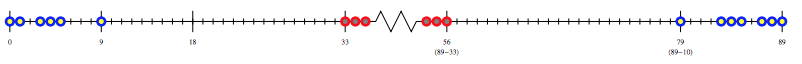
\includegraphics[scale=.7]{middle_colored.png}
        \label{fig:middle}
    \end{figure}
    \pause

    \item The fringes maintain their shape when added and subtracted, but after enough additions and subtractions, the middle will cover the holes in the fringes.
\end{itemize}

\end{frame}

%%%%%%%%%%%%%%%%%%%%%%%%%%%%%%%%%%%%%%%%%%%%%%%%%%%%%%%%%%%%%%%%%%%%%%%%%%%%%%%

\begin{frame}{2-Dimensional Constructions}

How do the $1$-dimensional constructions generalize to $2$-dimensions?
\pause

\begin{figure}
    \centering
    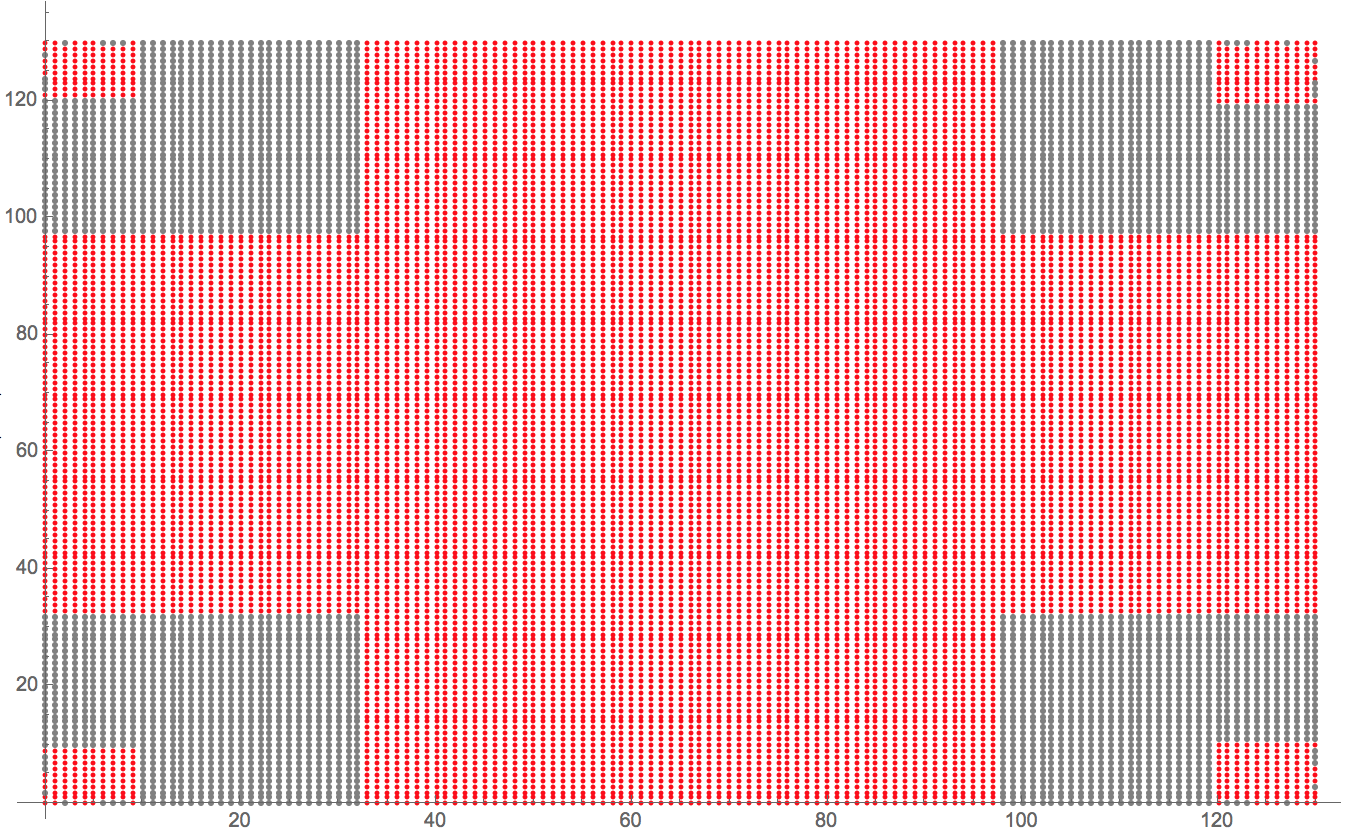
\includegraphics[scale=.35]{generalized_MSTD_set.png}
    \caption{$2$-dimensional generalized MSTD set}
    \label{fig:2dGenMSTD}
\end{figure}

\end{frame}

%%%%%%%%%%%%%%%%%%%%%%%%%%%%%%%%%%%%%%%%%%%%%%%%%%%%%%%%%%%%%%%%%%%%%%%%%%%%%%%

\begin{frame}{2-Dimensional Constructions}

How do the $1$-dimensional constructions generalize to $2$-dimensions?

\pause
\begin{figure}
    \centering
    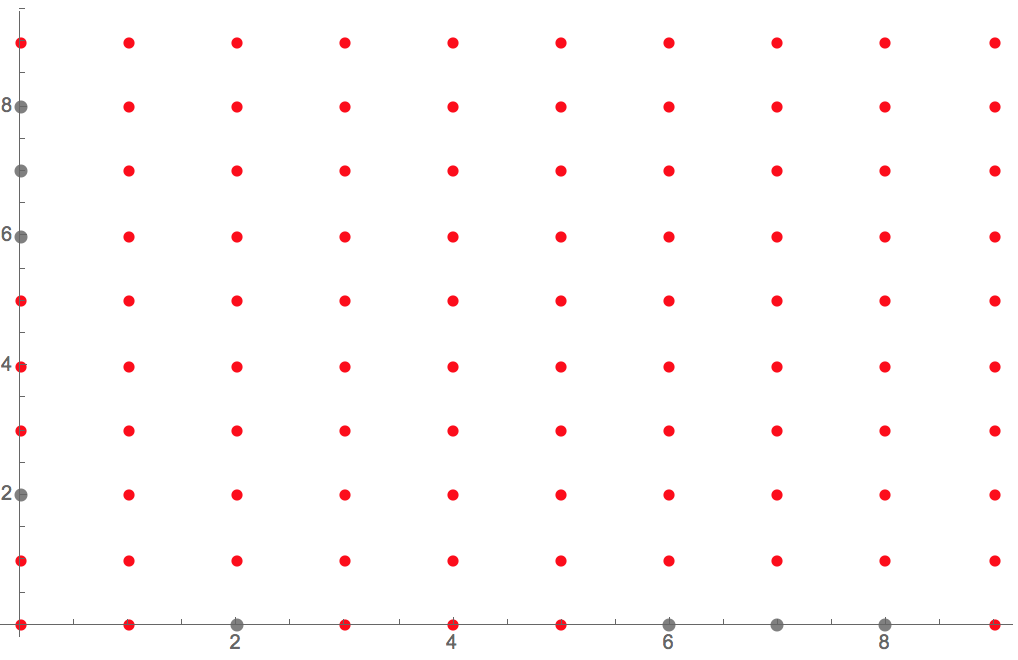
\includegraphics[scale=.45]{fringe_set.png}
    \caption{Zooming into the fringe in the corner}
    \label{fig:2dFringe}
\end{figure}

\end{frame}

%%%%%%%%%%%%%%%%%%%%%%%%%%%%%%%%%%%%%%%%%%%%%%%%%%%%%%%%%%%%%%%%%%%%%%%%%%%%%%%
%%%%%%%%%%%%%%%%%%%%%%%%%%%%%%%%%%%%%%%%%%%%%%%%%%%%%%%%%%%%%%%%%%%%%%%%%%%%%%%
\section{Generations} %elena
%%%%%%%%%%%%%%%%%%%%%%%%%%%%%%%%%%%%%%%%%%%%%%%%%%%%%%%%%%%%%%%%%%%%%%%%%%%%%%%
%%%%%%%%%%%%%%%%%%%%%%%%%%%%%%%%%%%%%%%%%%%%%%%%%%%%%%%%%%%%%%%%%%%%%%%%%%%%%%%

\begin{frame}{$k$-Generational Sets}

\begin{itemize}

\item Using this construction, for $s_1+d_1=s_2+d_2=k$ we can find a set $A \subset \Z^2$ such that $|s_1A-d_1A|>|s_2A-d_2A|$.

\pause
\Bigskip

\item We can prove that for any $x_1+y_1=x_2+y_2 \neq k$, we have $|x_1A-y_1A|=|x_2A-y_2A|$.

\pause
\Bigskip

\item We can then use these sets to create a set $A'\subset \Z^2$ such that $|cA'+cA'|>|cA'-cA'|$ for all $1\leq c \leq k.$ These sets are known as \emph{$k$-generational}.

\pause
\Bigskip

\item To construct $k$-generational sets, we will need to introduce \emph{base expansion}.

\end{itemize}

\end{frame}

%%%%%%%%%%%%%%%%%%%%%%%%%%%%%%%%%%%%%%%%%%%%%%%%%%%%%%%%%%%%%%%%%%%%%%%%%%%%%%%

\begin{frame}{Base Expansion}

Idea behind base expansion:

\pause
\Bigskip

\begin{itemize}
\item
For sets $A,B \subset \Z^2$ and $m\in \N$ sufficiently large (relative to $A$) we define:
$$C=m\cdot A+B$$
\pause

\item We have proved
$$\left|sC - dC\right|=\left|sA - dA\right|\cdot\left|sB - dB\right|.$$

\end{itemize}

\end{frame}

%%%%%%%%%%%%%%%%%%%%%%%%%%%%%%%%%%%%%%%%%%%%%%%%%%%%%%%%%%%%%%%%%%%%%%%%%%%%%%%

\begin{frame}{$k$-Generational Existence}

\textbf{Recall: } A set $A$ such that $|cA+cA|>|cA-cA|$ for all $1\leq c \leq k$ is \emph{$k$-generational}.

%\begin{theorem}
%Let $x_j, y_j, w_j, z_j$ be finite sequences of non-negative integers of length $k$ such that $x_j +y_j=w_j +z_j=j,$ and $\{x_j, y_j\} \neq \{w_j, z_j\}$ for every $2 \leq j \leq k.$ There exists a  $2$-dimensional set A that satisfies $|x_jA-y_jA| >|w_jA-z_jA|$ for every $2 \leq j \leq k.$
%\end{theorem}

%\pause
%\medskip

%$k$-generational sets are when $x_j=2j$, $y_j=0$, $w_j=z_j=j$.

\pause
\Bigskip

For each $i$, choose $A_{i}$ with $\left|iA_{i}+iA_{i}\right|$ $>$ $\left|iA_{i}-iA_{i}\right|$
and $|jA_{i}$ $+$ $jA_{i}|$ $=$ $|jA_{i}$ $-$ $jA_{i}|$.

\pause
\Bigskip

Define $A=A_{1}+mA_{2}+m^{2}A_{3}+\cdots+m^{k-1}A_{k}$.

\end{frame}

%%%%%%%%%%%%%%%%%%%%%%%%%%%%%%%%%%%%%%%%%%%%%%%%%%%%%%%%%%%%%%%%%%%%%%%%%%%%%%%

\begin{frame}{$k$-Generational Existence}

Define $A=A_{1}+mA_{2}+m^{2}A_{3}+\cdots+m^{k-1}A_{k}$.

\vspace{-\baselineskip}

\begin{eqnarray*}
	\left| jA+jA\right| \ &=& \ \prod_{i=1}^{k}\left|jA_{i}+jA_{i} \right| \pause \\
	 \ &=& \ \left|jA_{j}+jA_{j}\right|\cdot\prod_{i\neq j}\left|jA_{i}+jA_{i}\right|\pause \\
	 \ &=& \ \left|jA_{j}+jA_{j}\right|\cdot\prod_{i\neq j}\left|jA_{i}-jA_{i}\right|\pause \\ 
	 \ &>& \ \left|jA_{j}-jA_{j}\right|\cdot\prod_{i\neq j}\left|jA_{i}-jA_{i}\right|\pause \\
	 \ &=& \ \left|jA-jA\right|.
\end{eqnarray*}
    
\end{frame}

%%%%%%%%%%%%%%%%%%%%%%%%%%%%%%%%%%%%%%%%%%%%%%%%%%%%%%%%%%%%%%%%%%%%%%%%%%%%%%%

\begin{frame}{Limiting Behavior of $kA$}
Are there any $2$-dimensional sets such that $|kA+kA|>|kA-kA|$ for all  $k \in \N$? 

\pause

\bigskip
First we have to describe the behavior of $kA$.
\pause

\bigskip
\begin{theorem}[Nathanson]\label{Nathanson}
Let $A=\{a_0, a_1, \ldots, a_k\}$ be a finite set of integers with $a_0=0<a_1 < \cdots < a_m=a$ and $(a_1, a_2, \ldots, a_m)=1.$ Then there exists non-negative integers $c$ and $d$ and sets $C\subset [0, c-2]$ and $D\subset [0,d-2]$ such that for all $k \geq a^2m$, $$kA \ = \ C \cup [c, ka-d] \cup ka-D$$
\end{theorem}

\end{frame}

%%%%%%%%%%%%%%%%%%%%%%%%%%%%%%%%%%%%%%%%%%%%%%%%%%%%%%%%%%%%%%%%%%%%%%%%%%%%%%%

\begin{frame}{Limiting Behavior of $kA$}

\begin{theorem} \label{growth of kA-1}
Let $A\subset \Z^2$. Let $a$ and $b$ be the smallest non-zero $x$ and $y$ coordinates, $a'$ and $b'$ be the largest $x$ and $y$ coordinates, and $N=\max\{2a'^2, 2b'^2\}$. If $(a, a')=0$, $(b,b')=0$, and $\color{red}\{(0,0), (a,0), (0,b), (a',0),(0,b'),(a,b),$

$\color{red} (a,b'),(a',b), (a',b') \} \subset A$,  then for $k \geq N$  and for some constants $C, c_1, c_2$, we have $\color{red}|kA|=k^2a'b' -C-c_1k -c_2k$. 
\end{theorem}

\end{frame}

%%%%%%%%%%%%%%%%%%%%%%%%%%%%%%%%%%%%%%%%%%%%%%%%%%%%%%%%%%%%%%%%%%%%%%%%%%%%%%%

\begin{frame}{Limiting Behavior of $kA$}
We want to show for sufficiently large $k$, the amount of elements missing from $kA$ grows linearly.

\pause

\begin{figure}
    \centering
    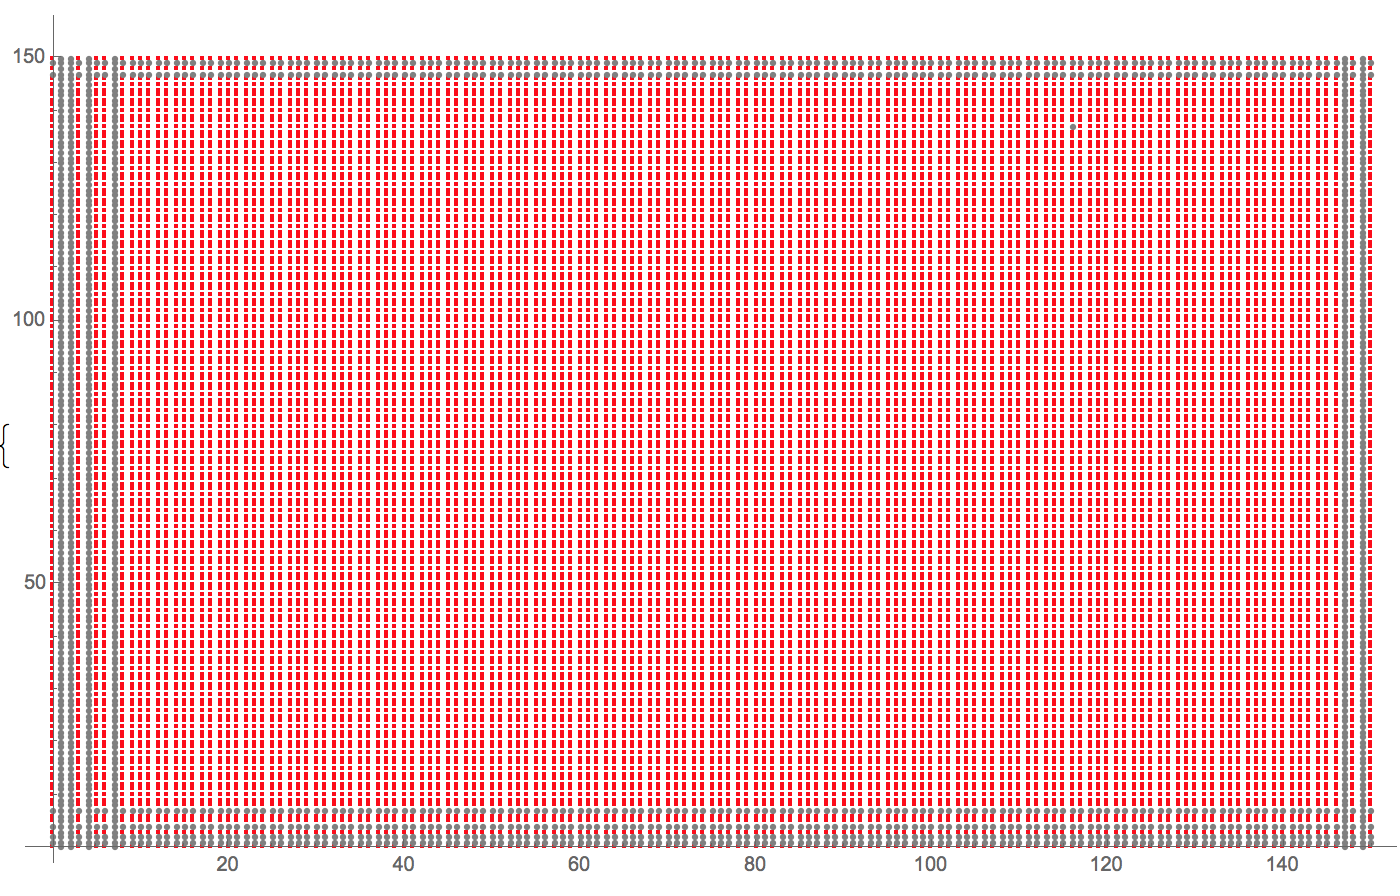
\includegraphics[scale=.35]{stabilized_set.png}
    \label{fig:stablized set-1}
\end{figure}

\end{frame}

%%%%%%%%%%%%%%%%%%%%%%%%%%%%%%%%%%%%%%%%%%%%%%%%%%%%%%%%%%%%%%%%%%%%%%%%%%%%%%%

\begin{frame}{$|kA-kA| \geq |kA+kA|$}
\begin{theorem} \label{growth of kA-2}
Let $A \subset \Z^2$. Let $a$ and $b$ be the smallest non-zero $x$ and $y$ coordinates, $a'$ and $b'$ be the largest $x$ and $y$ coordinates, and $N=\max\{2a'^2, 2b'^2\}$. If $(a, a')=0$, $(b,b')=0$, and $\{(0,0), (a,0), (0,b), (a',0),(0,b'),(a,b),$

$(a,b'),(a',b), (a',b') \} \subset A$, then for $k \geq N$, we have $\color{red} |kA-kA| \geq |kA+kA|$. 
\end{theorem}


    
\end{frame}

%%%%%%%%%%%%%%%%%%%%%%%%%%%%%%%%%%%%%%%%%%%%%%%%%%%%%%%%%%%%%%%%%%%%%%%%%%%%%%%
\begin{frame}{$|kA-kA| \geq |kA+kA|$}

We want to show $|kA-kA| \geq |kA+kA|$.

\pause

\begin{figure}
    \centering
    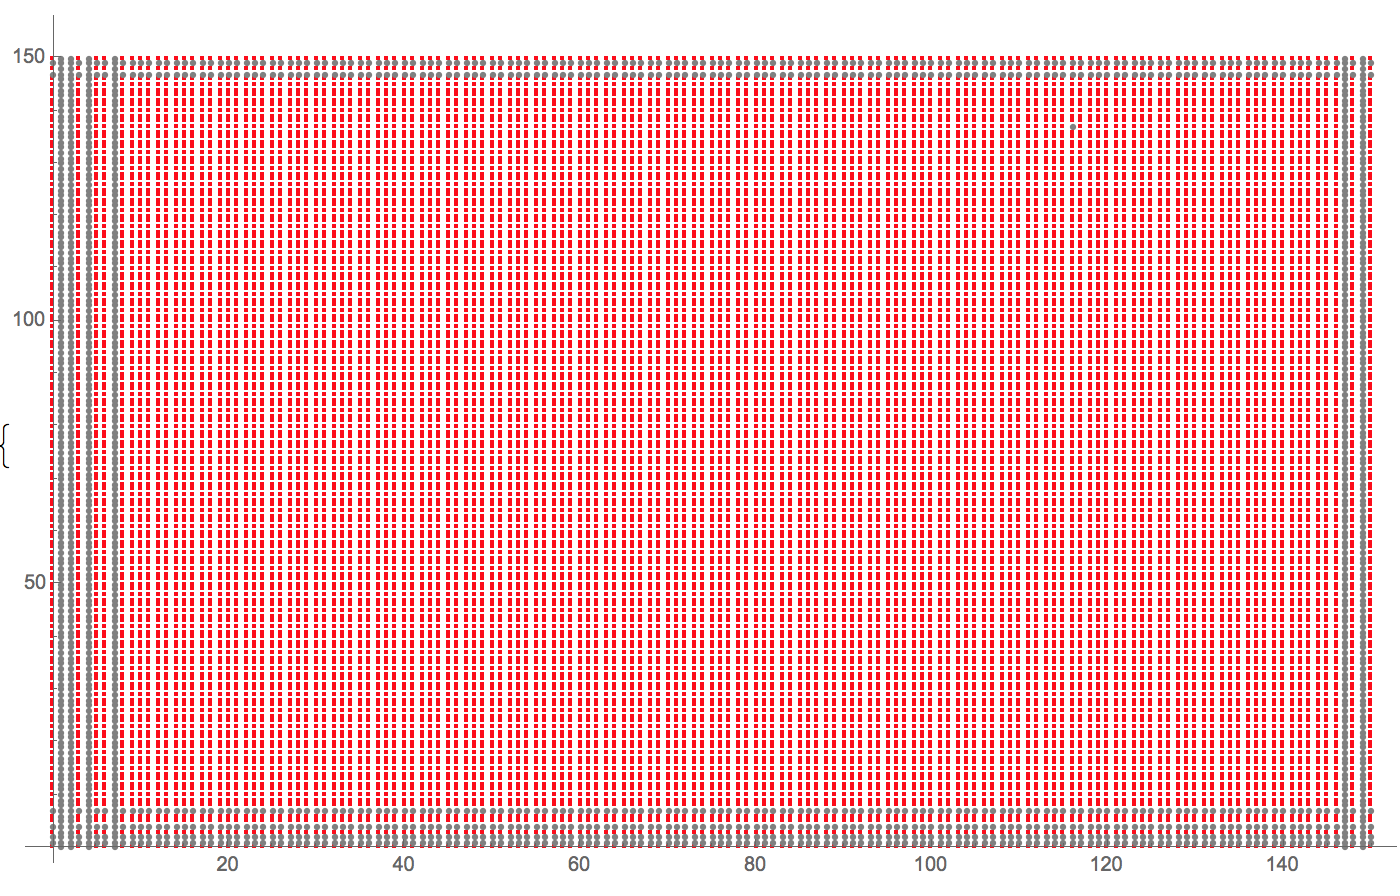
\includegraphics[scale=.35]{stabilized_set.png}
    \label{fig:stablized set-2}
\end{figure}
    
\end{frame}

%%%%%%%%%%%%%%%%%%%%%%%%%%%%%%%%%%%%%%%%%%%%%%%%%%%%%%%%%%%%%%%%%%%%%%%%%%%%%%%
%%%%%%%%%%%%%%%%%%%%%%%%%%%%%%%%%%%%%%%%%%%%%%%%%%%%%%%%%%%%%%%%%%%%%%%%%%%%%%%
\section{Other Constructions}
%%%%%%%%%%%%%%%%%%%%%%%%%%%%%%%%%%%%%%%%%%%%%%%%%%%%%%%%%%%%%%%%%%%%%%%%%%%%%%%
%%%%%%%%%%%%%%%%%%%%%%%%%%%%%%%%%%%%%%%%%%%%%%%%%%%%%%%%%%%%%%%%%%%%%%%%%%%%%%%

\begin{frame}{$d$-Dimensional Constructions}
What does the middle look like in $d$-dimensions?

\bigskip
\pause

\begin{center}
    \tdplotsetmaincoords{60}{45}
    \begin{tikzpicture}[tdplot_main_coords, scale=0.75]
        \newcommand{\drawcross}{
        	\clip 
        		(1.5, 1.5) rectangle (3.5, 3.5)
        		(1.5, 0) rectangle (3.5, 1.5)
        		(3.5, 1.5) rectangle (5, 3.5)
        		(3.5, 5) rectangle (1.5, 3.5)
        		(1.5, 3.5) rectangle (0, 1.5);
        	\fill[umichblue]
        		(1.5, 1.5) rectangle (3.5, 3.5)
        		(1.5, 0) rectangle (3.5, 1.5)
        		(3.5, 1.5) rectangle (5, 3.5)
        		(3.5, 5) rectangle (1.5, 3.5)
        		(1.5, 3.5) rectangle (0, 1.5);
        	\draw[thick]
        		(1.5, 0) -- (3.5, 0)
        			   -- (3.5, 1.5)
        			   -- (5, 1.5)
        			   -- (5, 3.5)
        			   -- (3.5, 3.5)
        			   -- (3.5, 5)
        			   -- (1.5, 5)
        			   -- (1.5, 3.5)
        			   -- (0, 3.5)
        			   -- (0, 1.5)
        			   -- (1.5, 1.5)
        			   -- cycle;
        }
        
        \newcommand{\drawcorners}{
        	\clip (0, 0) rectangle (5, 5);
        	\fill[umichmaize]
        		(0, 0) rectangle (1.5, 1.5)
        		(3.5, 0) rectangle (5, 1.5)
        		(3.5, 3.5) rectangle (5, 5)
        		(1.5, 3.5) rectangle (0, 5);
        	\draw[thick]
        		(0, 0) rectangle (1.5, 1.5)
        		(3.5, 0) rectangle (5, 1.5)
        		(3.5, 3.5) rectangle (5, 5)
        		(1.5, 3.5) rectangle (0, 5);
        }
        
        \begin{scope}[canvas is xz plane at y=1.5]
        	\drawcorners
        \end{scope}
        
        \begin{scope}[canvas is xy plane at z=3.5]
        	\drawcorners
        \end{scope}
        
        \begin{scope}[canvas is yz plane at x=3.5]
        	\drawcorners
        \end{scope}
        
        \begin{scope}[canvas is xz plane at y=0]
        	\drawcross
        \end{scope}
        
        \begin{scope}[canvas is xy plane at z=5]
        	\drawcross
        \end{scope}
        
        \begin{scope}[canvas is yz plane at x=5]
        	\drawcross
        \end{scope}
    \end{tikzpicture}
\end{center}

% For $s_1>s_2$,
% $$M \ = \ \bigcup_{i=1}^d \left\{(x_1, x_2, \ldots, x_d): \substack{2k^2+1-d_1 \leq x_j \leq n_j- (2k^2+1-d_1) \text{ for } j \neq i,\\0\leq x_i \leq n_i} \right\}$$
%
% \pause
%
% For $s_2>s_1$,
% $$M \ = \ \bigcup_{i=1}^d \left\{(x_1, x_2, \ldots, x_d): \substack{2k^2+1-s_1 \leq x_j \leq n_j- (2k^2+1-s_1) \text{ for } j \neq i,\\0 \leq x_i \leq n_i} \right\}$$

\end{frame}

%%%%%%%%%%%%%%%%%%%%%%%%%%%%%%%%%%%%%%%%%%%%%%%%%%%%%%%%%%%%%%%%%%%%%%%%%%%%%%%

\begin{frame}{$d$-Dimensional Constructions}
What do the fringes look like in $d$-dimensions?
\pause
\bigskip

\begin{center}
    \tdplotsetmaincoords{60}{45}
    \begin{tikzpicture}[tdplot_main_coords]
        \begin{scope}[canvas is xz plane at y=0]
        	\clip (0, 0) rectangle (3, 3);
        	\fill[umichmaize] (0, 0) rectangle (3, 3);
        	\draw[thick] (0, 0) rectangle (3, 3);
        \end{scope}
        
        \begin{scope}[canvas is xy plane at z=3]
        	\clip (0, 0) rectangle (3, 3);
        	\fill[umichmaize] (0, 0) rectangle (3, 3);
        	\draw[thick] (0, 0) rectangle (3, 3);
        \end{scope}
        
        \begin{scope}[canvas is yz plane at x=3]
        	\clip (0, 0) rectangle (3, 3);
        	\fill[umichmaize] (0, 0) rectangle (3, 3);
        	\draw[thick] (0, 0) rectangle (3, 3);
        \end{scope}
        
        \foreach \val in {0, 1, 4/3, 5/3, 2, 8/3, 3} {
        	\draw[mark=*, mark size=2.5, only marks] plot coordinates {
        		(3, 0, \val)
        		(3, 3 - \val, 3)
        		(\val, 0, 3)
        	};
        }
        
    \end{tikzpicture}
\end{center}

% \small{
% \begin{align*}
% B_1 \ &= \ \{(x_1,0, \ldots, 0), \ldots, (0,0, \ldots, x_d): 0 \leq x_1, \ldots, x_d \leq 2k+1\}\setminus\\
% &\qquad\{(2,0, \ldots, 0), (0,2, \ldots, 0),  \ldots, (0,0, \ldots, 2)\} \cup\\
% &\qquad\{ (x_1, 0, \ldots, 0), (0, x_2, \ldots, 0), \ldots,  (0, 0, \ldots, x_d)\\
% &\hspace{2in}: k+2 \leq x_1, x_2, \ldots x_d \leq 2k\}
% \end{align*}
%
% \begin{align*}
% B_2 \ &= \ \{(x_1,0, \ldots, 0), \ldots, (0,0, \ldots, x_d): 0 \leq x_1, \ldots, x_d \leq 2k+2\}\setminus\\
% &\qquad \{(3,0, \ldots, 0), (0,3, \ldots, 0),  \ldots, (0,0, \ldots, 3)\} \cup\\
% &\qquad \{ (x_1, 0, \ldots, 0), (0, x_2, \ldots, 0), \ldots,  (0, 0, \ldots, x_d)\\
% &\hspace{2in}: k+3 \leq x_1, x_2, \ldots x_d \leq 2k+1\}.
% \end{align*}
% }

\end{frame}

%%%%%%%%%%%%%%%%%%%%%%%%%%%%%%%%%%%%%%%%%%%%%%%%%%%%%%%%%%%%%%%%%%%%%%%%%%%%%%%
\begin{frame}{Other 2-Dimensional Constructions}

Needs to  have integer vertices and be locally point symmetric.

\pause
\bigskip

Parallelogram with slope $m$.

\pause 
\bigskip

Define $\varphi: \Z^2 \to \Z^2$ by $\varphi(x,y)= (x+my, y).$ 

\pause

\begin{figure}
    \centering
    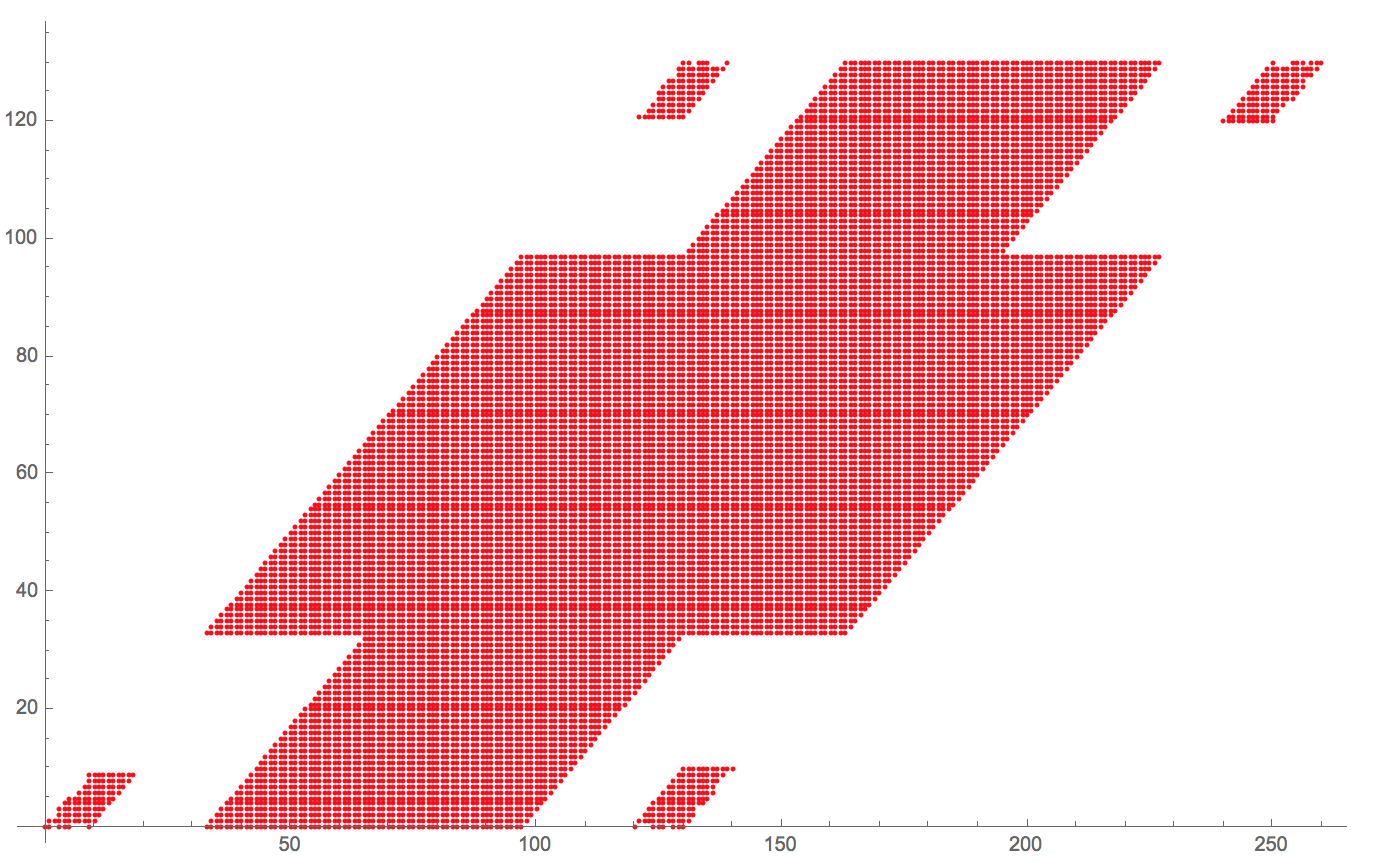
\includegraphics[scale=.2]{parallelogram.png}
    \caption{The generalized MSTD set for $k=4$, $n=130,$ $s_1=4$, $d_1=0$, $s_2=2$, and $d_2=2$ that has been sheared with slope $m=1$}
    \label{fig:my_label}
\end{figure}

\end{frame}

%%%%%%%%%%%%%%%%%%%%%%%%%%%%%%%%%%%%%%%%%%%%%%%%%%%%%%%%%%%%%%%

\begin{frame}{Parallelogram $d$-Dimensional Constructions}
\begin{itemize}
    \item $d(d-1)/2$ positive directions to shear the set 
    
    \pause
    \bigskip
    
    \item  $d(d-1)/2$ slopes:
        $$m_{1,2}, m_{1,2}, \ldots, m_{1,d}, m_{2,3}, \ldots, m_{2,d}, \ldots, m_{d-1,d}$$
        \pause
        ($m_{i,j}$ is the $j$th axis sheared in the $i$th direction)
    
    \pause
    \bigskip
    
    \item We define $\psi: \Z^2 \to \Z^2d$ by 
        \begin{align*}
            \psi(x_1, x_2, \ldots, x_d) \ &= \ (x_1 +m_{1,2}x_2 + m_{1,3}x_3 + \ldots + m_{1,d}x_d,\\
            &\qquad\quad x_2 +m_{2,3}x_3  + \ldots + m_{2,d}x_d, \ldots, x_d).
        \end{align*}
\end{itemize}

\end{frame}


%%%%%%%%%%%%%%%%%%%%%%%%%%%%%%%%%%%%%%%%%%%%%%%%%%%%%%%%%%%%%%%%%%%%%%%%%%%%%%%
%%%%%%%%%%%%%%%%%%%%%%%%%%%%%%%%%%%%%%%%%%%%%%%%%%%%%%%%%%%%%%%%%%%%%%%%%%%%%%%
\section{Conclusion}
%%%%%%%%%%%%%%%%%%%%%%%%%%%%%%%%%%%%%%%%%%%%%%%%%%%%%%%%%%%%%%%%%%%%%%%%%%%%%%%
%%%%%%%%%%%%%%%%%%%%%%%%%%%%%%%%%%%%%%%%%%%%%%%%%%%%%%%%%%%%%%%%%%%%%%%%%%%%%%%

\begin{frame}{Future Directions}
\begin{itemize}
    \item We have shown the elements missing from $kA$ grows linearly for certain $A$ 
    
    \pause
    \bigskip
    
    \item \textbf{In the future: } show that the elements missing from  $kA$ grows linearly for all $A$ 
    
    \pause
    \bigskip
    
    \item Previous work in $1$-dimensions has shown positive percentages for generalized MSTD sets, chains of generalized MSTD sets, and $k$-generational sets
    
    \pause
    \bigskip
    
    \item \textbf{In the future: } Show positive percentages for $d$-dimensional sets
\end{itemize}

\end{frame}

%%%%%%%%%%%%%%%%%%%%%%%%%%%%%%%%%%%%%%%%%%%%%%%%%%%%%%%%%%%%%%%%%%%%%%%%%%%%%%%

\begin{frame}{Thanks}

Thanks to:
\begin{itemize}
\item Our mentor Prof. Steven Miller,
    \smallskip
\item Williams College,
    \smallskip
\item Yale University,
    \smallskip
\item NSF Grants DMS1947438 and DMS1561945,
    \smallskip
\item YMC Coordinators.
\end{itemize}

\end{frame}

%%%%%%%%%%%%%%%%%%%%%%%%%%%%%%%%%%%%%%%%%%%%%%%%%%%%%%%%%%%%%%%%%%%%%%%%%%%%%%%
%%%%%%%%%%%%%%%%%%%%%%%%%%%%%%%%%%%%%%%%%%%%%%%%%%%%%%%%%%%%%%%%%%%%%%%%%%%%%%%
%%%%%%%%%%%%%%%%%%%%%%%%%%%%%%%%%%%%%%%%%%%%%%%%%%%%%%%%%%%%%%%%%%%%%%%%%%%%%%%
%%%%%%%%%%%%%%%%%%%%%%%%%%%%%%%%%%%%%%%%%%%%%%%%%%%%%%%%%%%%%%%%%%%%%%%%%%%%%%%
\end{document}
